\documentclass[twoside]{book}

% Packages required by doxygen
\usepackage{calc}
\usepackage{doxygen}
\usepackage{graphicx}
\usepackage[utf8]{inputenc}
\usepackage{makeidx}
\usepackage{multicol}
\usepackage{multirow}
\usepackage{fixltx2e}
\PassOptionsToPackage{warn}{textcomp}
\usepackage{textcomp}
\usepackage[nointegrals]{wasysym}
\usepackage[table]{xcolor}

% Font selection
\usepackage[T1]{fontenc}
\usepackage{mathptmx}
\usepackage[scaled=.90]{helvet}
\usepackage{courier}
\usepackage{amssymb}
\usepackage{sectsty}
\renewcommand{\familydefault}{\sfdefault}
\allsectionsfont{%
  \fontseries{bc}\selectfont%
  \color{darkgray}%
}
\renewcommand{\DoxyLabelFont}{%
  \fontseries{bc}\selectfont%
  \color{darkgray}%
}
\newcommand{\+}{\discretionary{\mbox{\scriptsize$\hookleftarrow$}}{}{}}

% Page & text layout
\usepackage{geometry}
\geometry{%
  a4paper,%
  top=2.5cm,%
  bottom=2.5cm,%
  left=2.5cm,%
  right=2.5cm%
}
\tolerance=750
\hfuzz=15pt
\hbadness=750
\setlength{\emergencystretch}{15pt}
\setlength{\parindent}{0cm}
\setlength{\parskip}{0.2cm}
\makeatletter
\renewcommand{\paragraph}{%
  \@startsection{paragraph}{4}{0ex}{-1.0ex}{1.0ex}{%
    \normalfont\normalsize\bfseries\SS@parafont%
  }%
}
\renewcommand{\subparagraph}{%
  \@startsection{subparagraph}{5}{0ex}{-1.0ex}{1.0ex}{%
    \normalfont\normalsize\bfseries\SS@subparafont%
  }%
}
\makeatother

% Headers & footers
\usepackage{fancyhdr}
\pagestyle{fancyplain}
\fancyhead[LE]{\fancyplain{}{\bfseries\thepage}}
\fancyhead[CE]{\fancyplain{}{}}
\fancyhead[RE]{\fancyplain{}{\bfseries\leftmark}}
\fancyhead[LO]{\fancyplain{}{\bfseries\rightmark}}
\fancyhead[CO]{\fancyplain{}{}}
\fancyhead[RO]{\fancyplain{}{\bfseries\thepage}}
\fancyfoot[LE]{\fancyplain{}{}}
\fancyfoot[CE]{\fancyplain{}{}}
\fancyfoot[RE]{\fancyplain{}{\bfseries\scriptsize Generated on Fri Dec 5 2014 21\+:35\+:22 for My Project by Doxygen }}
\fancyfoot[LO]{\fancyplain{}{\bfseries\scriptsize Generated on Fri Dec 5 2014 21\+:35\+:22 for My Project by Doxygen }}
\fancyfoot[CO]{\fancyplain{}{}}
\fancyfoot[RO]{\fancyplain{}{}}
\renewcommand{\footrulewidth}{0.4pt}
\renewcommand{\chaptermark}[1]{%
  \markboth{#1}{}%
}
\renewcommand{\sectionmark}[1]{%
  \markright{\thesection\ #1}%
}

% Indices & bibliography
\usepackage{natbib}
\usepackage[titles]{tocloft}
\setcounter{tocdepth}{3}
\setcounter{secnumdepth}{5}
\makeindex

% Hyperlinks (required, but should be loaded last)
\usepackage{ifpdf}
\ifpdf
  \usepackage[pdftex,pagebackref=true]{hyperref}
\else
  \usepackage[ps2pdf,pagebackref=true]{hyperref}
\fi
\hypersetup{%
  colorlinks=true,%
  linkcolor=blue,%
  citecolor=blue,%
  unicode%
}

% Custom commands
\newcommand{\clearemptydoublepage}{%
  \newpage{\pagestyle{empty}\cleardoublepage}%
}


%===== C O N T E N T S =====

\begin{document}

% Titlepage & ToC
\hypersetup{pageanchor=false,
             bookmarks=true,
             bookmarksnumbered=true,
             pdfencoding=unicode
            }
\pagenumbering{roman}
\begin{titlepage}
\vspace*{7cm}
\begin{center}%
{\Large My Project }\\
\vspace*{1cm}
{\large Generated by Doxygen 1.8.7}\\
\vspace*{0.5cm}
{\small Fri Dec 5 2014 21:35:22}\\
\end{center}
\end{titlepage}
\clearemptydoublepage
\tableofcontents
\clearemptydoublepage
\pagenumbering{arabic}
\hypersetup{pageanchor=true}

%--- Begin generated contents ---
\chapter{Hierarchical Index}
\section{Class Hierarchy}
This inheritance list is sorted roughly, but not completely, alphabetically\+:\begin{DoxyCompactList}
\item Comparable\begin{DoxyCompactList}
\item \contentsline{section}{Vertex}{\pageref{class_vertex}}{}
\end{DoxyCompactList}
\item \contentsline{section}{Dijkstra}{\pageref{class_dijkstra}}{}
\item \contentsline{section}{Edge}{\pageref{class_edge}}{}
\item \contentsline{section}{Find\+Shortest\+Road\+Path}{\pageref{class_find_shortest_road_path}}{}
\item \contentsline{section}{Graph}{\pageref{class_graph}}{}
\item \contentsline{section}{Graph\+Initializer}{\pageref{class_graph_initializer}}{}
\end{DoxyCompactList}

\chapter{Class Index}
\section{Class List}
Here are the classes, structs, unions and interfaces with brief descriptions\+:\begin{DoxyCompactList}
\item\contentsline{section}{\hyperlink{class_dijkstra}{Dijkstra} }{\pageref{class_dijkstra}}{}
\item\contentsline{section}{\hyperlink{class_edge}{Edge} }{\pageref{class_edge}}{}
\item\contentsline{section}{\hyperlink{class_find_shortest_road_path}{Find\+Shortest\+Road\+Path} }{\pageref{class_find_shortest_road_path}}{}
\item\contentsline{section}{\hyperlink{class_graph}{Graph} }{\pageref{class_graph}}{}
\item\contentsline{section}{\hyperlink{class_graph_initializer}{Graph\+Initializer} }{\pageref{class_graph_initializer}}{}
\item\contentsline{section}{\hyperlink{class_vertex}{Vertex} }{\pageref{class_vertex}}{}
\end{DoxyCompactList}

\chapter{File Index}
\section{File List}
Here is a list of all documented files with brief descriptions\+:\begin{DoxyCompactList}
\item\contentsline{section}{\hyperlink{_find_shortest_road_path_8java}{Find\+Shortest\+Road\+Path.\+java} \\*Class \hyperlink{class_find_shortest_road_path}{Find\+Shortest\+Road\+Path} is used to gather user input data and initialize the graph. It will then perform \hyperlink{class_dijkstra}{Dijkstra}'s Algorithm on the graph and save the results to a text file }{\pageref{_find_shortest_road_path_8java}}{}
\item\contentsline{section}{\hyperlink{_graph_8java}{Graph.\+java} \\*Class \hyperlink{class_graph}{Graph} defines a graph that is made of vertexes and edges, the underlying implementation is a hashmap }{\pageref{_graph_8java}}{}
\item\contentsline{section}{\hyperlink{_graph_initializer_8java}{Graph\+Initializer.\+java} \\*Class \hyperlink{class_graph_initializer}{Graph\+Initializer} is used to fill the \hyperlink{class_graph}{Graph} with the data from input files }{\pageref{_graph_initializer_8java}}{}
\item\contentsline{section}{\hyperlink{_vertex_8java}{Vertex.\+java} \\*Class \hyperlink{class_vertex}{Vertex} defines a \hyperlink{class_vertex}{Vertex} in relation to a \hyperlink{class_graph}{Graph} }{\pageref{_vertex_8java}}{}
\end{DoxyCompactList}

\chapter{Class Documentation}
\hypertarget{class_dijkstra}{\section{Dijkstra Class Reference}
\label{class_dijkstra}\index{Dijkstra@{Dijkstra}}
}
\subsection*{Static Public Member Functions}
\begin{DoxyCompactItemize}
\item 
\hypertarget{class_dijkstra_a51d03e229ce98b3ef56dc1ceb178192f}{static void {\bfseries compute\+Paths} (\hyperlink{class_vertex}{Vertex} source, \hyperlink{class_graph}{Graph} graph)}\label{class_dijkstra_a51d03e229ce98b3ef56dc1ceb178192f}

\item 
\hypertarget{class_dijkstra_a5c7efba36207a7884685b07854459090}{static Array\+List$<$ String $>$ {\bfseries get\+Shortest\+Path\+To} (\hyperlink{class_vertex}{Vertex} target, \hyperlink{class_vertex}{Vertex} source, \hyperlink{class_graph}{Graph} graph)}\label{class_dijkstra_a5c7efba36207a7884685b07854459090}

\end{DoxyCompactItemize}


The documentation for this class was generated from the following file\+:\begin{DoxyCompactItemize}
\item 
Dijkstra.\+java\end{DoxyCompactItemize}

\hypertarget{class_edge}{\section{Edge Class Reference}
\label{class_edge}\index{Edge@{Edge}}
}
\subsection*{Public Member Functions}
\begin{DoxyCompactItemize}
\item 
\hypertarget{class_edge_a2e0bc2ab99efaff142522be150f0d010}{{\bfseries Edge} (String target, int weight)}\label{class_edge_a2e0bc2ab99efaff142522be150f0d010}

\item 
\hypertarget{class_edge_a1157117272aaebf06828ab52e915b100}{String {\bfseries get\+Target} ()}\label{class_edge_a1157117272aaebf06828ab52e915b100}

\item 
\hypertarget{class_edge_a963d963b098f2329738cde01942be520}{int {\bfseries get\+Weight} ()}\label{class_edge_a963d963b098f2329738cde01942be520}

\end{DoxyCompactItemize}


The documentation for this class was generated from the following file\+:\begin{DoxyCompactItemize}
\item 
Edge.\+java\end{DoxyCompactItemize}

\hypertarget{class_find_shortest_road_path}{\section{Find\+Shortest\+Road\+Path Class Reference}
\label{class_find_shortest_road_path}\index{Find\+Shortest\+Road\+Path@{Find\+Shortest\+Road\+Path}}
}
\subsection*{Static Public Member Functions}
\begin{DoxyCompactItemize}
\item 
\hypertarget{class_find_shortest_road_path_a4c742064cbfb91124a1fc7126103b425}{static void {\bfseries main} (String\mbox{[}$\,$\mbox{]} args)}\label{class_find_shortest_road_path_a4c742064cbfb91124a1fc7126103b425}

\end{DoxyCompactItemize}


The documentation for this class was generated from the following file\+:\begin{DoxyCompactItemize}
\item 
\hyperlink{_find_shortest_road_path_8java}{Find\+Shortest\+Road\+Path.\+java}\end{DoxyCompactItemize}

\hypertarget{class_graph}{\section{Graph Class Reference}
\label{class_graph}\index{Graph@{Graph}}
}
\subsection*{Public Member Functions}
\begin{DoxyCompactItemize}
\item 
\hypertarget{class_graph_a057fcdd662a72caa686d040b003b3965}{void {\bfseries add\+Vertex} (String vertex\+I\+D, \hyperlink{class_edge}{Edge} edge)}\label{class_graph_a057fcdd662a72caa686d040b003b3965}

\item 
\hypertarget{class_graph_a1c30cb604ce468ee430eb55333844a04}{\hyperlink{class_vertex}{Vertex} {\bfseries get\+Vertex} (String vertex\+I\+D)}\label{class_graph_a1c30cb604ce468ee430eb55333844a04}

\item 
\hypertarget{class_graph_a628649853217f6c4c03679a0ee138dde}{boolean {\bfseries has\+Vertex} (String vertex\+I\+D)}\label{class_graph_a628649853217f6c4c03679a0ee138dde}

\item 
\hypertarget{class_graph_a007a1d7365127b0038175e04be7ee3e0}{int {\bfseries get\+Vertex\+Count} ()}\label{class_graph_a007a1d7365127b0038175e04be7ee3e0}

\item 
\hypertarget{class_graph_a1255a24915fbb017558ea54a197c8769}{Hash\+Map$<$ String, \hyperlink{class_vertex}{Vertex} $>$ {\bfseries get\+Vertex\+Map} ()}\label{class_graph_a1255a24915fbb017558ea54a197c8769}

\end{DoxyCompactItemize}


The documentation for this class was generated from the following file\+:\begin{DoxyCompactItemize}
\item 
\hyperlink{_graph_8java}{Graph.\+java}\end{DoxyCompactItemize}

\hypertarget{class_graph_initializer}{\section{Graph\+Initializer Class Reference}
\label{class_graph_initializer}\index{Graph\+Initializer@{Graph\+Initializer}}
}
\subsection*{Public Member Functions}
\begin{DoxyCompactItemize}
\item 
\hyperlink{class_graph_initializer_a4b294602437d6408c186890991a3e036}{Graph\+Initializer} (String input\+File)
\begin{DoxyCompactList}\small\item\em constructs the \hyperlink{class_graph_initializer}{Graph\+Initializer} \end{DoxyCompactList}\item 
\hyperlink{class_graph}{Graph} \hyperlink{class_graph_initializer_a82c569ac7cc45440e6d580754e3a3278}{create\+Graph} ()
\begin{DoxyCompactList}\small\item\em creates the graph with the Vertexes and their adjacent edges and distances \end{DoxyCompactList}\item 
\hyperlink{class_graph}{Graph} \hyperlink{class_graph_initializer_af0e556ec580f694932513607d847ad9a}{set\+Cordinates} (\hyperlink{class_graph}{Graph} graph, File cord\+File)
\begin{DoxyCompactList}\small\item\em assigns latitude and longitude cordinates to each \hyperlink{class_vertex}{Vertex} \end{DoxyCompactList}\end{DoxyCompactItemize}


\subsection{Constructor \& Destructor Documentation}
\hypertarget{class_graph_initializer_a4b294602437d6408c186890991a3e036}{\index{Graph\+Initializer@{Graph\+Initializer}!Graph\+Initializer@{Graph\+Initializer}}
\index{Graph\+Initializer@{Graph\+Initializer}!Graph\+Initializer@{Graph\+Initializer}}
\subsubsection[{Graph\+Initializer}]{\setlength{\rightskip}{0pt plus 5cm}Graph\+Initializer.\+Graph\+Initializer (
\begin{DoxyParamCaption}
\item[{String}]{input\+File}
\end{DoxyParamCaption}
)\hspace{0.3cm}{\ttfamily [inline]}}}\label{class_graph_initializer_a4b294602437d6408c186890991a3e036}


constructs the \hyperlink{class_graph_initializer}{Graph\+Initializer} 


\begin{DoxyParams}{Parameters}
{\em String} & input\+File which expects the input file containing the vertex data \\
\hline
\end{DoxyParams}


\subsection{Member Function Documentation}
\hypertarget{class_graph_initializer_a82c569ac7cc45440e6d580754e3a3278}{\index{Graph\+Initializer@{Graph\+Initializer}!create\+Graph@{create\+Graph}}
\index{create\+Graph@{create\+Graph}!Graph\+Initializer@{Graph\+Initializer}}
\subsubsection[{create\+Graph}]{\setlength{\rightskip}{0pt plus 5cm}{\bf Graph} Graph\+Initializer.\+create\+Graph (
\begin{DoxyParamCaption}
{}
\end{DoxyParamCaption}
)\hspace{0.3cm}{\ttfamily [inline]}}}\label{class_graph_initializer_a82c569ac7cc45440e6d580754e3a3278}


creates the graph with the Vertexes and their adjacent edges and distances 

\begin{DoxyReturn}{Returns}
\hyperlink{class_graph}{Graph} which is the newly created graph 
\end{DoxyReturn}
\hypertarget{class_graph_initializer_af0e556ec580f694932513607d847ad9a}{\index{Graph\+Initializer@{Graph\+Initializer}!set\+Cordinates@{set\+Cordinates}}
\index{set\+Cordinates@{set\+Cordinates}!Graph\+Initializer@{Graph\+Initializer}}
\subsubsection[{set\+Cordinates}]{\setlength{\rightskip}{0pt plus 5cm}{\bf Graph} Graph\+Initializer.\+set\+Cordinates (
\begin{DoxyParamCaption}
\item[{{\bf Graph}}]{graph, }
\item[{File}]{cord\+File}
\end{DoxyParamCaption}
)\hspace{0.3cm}{\ttfamily [inline]}}}\label{class_graph_initializer_af0e556ec580f694932513607d847ad9a}


assigns latitude and longitude cordinates to each \hyperlink{class_vertex}{Vertex} 


\begin{DoxyParams}{Parameters}
{\em \hyperlink{class_graph}{Graph}} & graph which expects the graph that is to have its Vertexes' cordinates set \\
\hline
{\em File} & cord\+File which expects the file containing the cordinates for the Vertexes \\
\hline
\end{DoxyParams}
\begin{DoxyReturn}{Returns}
\hyperlink{class_graph}{Graph} which is the newly created graph with cordinates 
\end{DoxyReturn}


The documentation for this class was generated from the following file\+:\begin{DoxyCompactItemize}
\item 
\hyperlink{_graph_initializer_8java}{Graph\+Initializer.\+java}\end{DoxyCompactItemize}

\hypertarget{class_vertex}{\section{Vertex Class Reference}
\label{class_vertex}\index{Vertex@{Vertex}}
}
Inheritance diagram for Vertex\+:\begin{figure}[H]
\begin{center}
\leavevmode
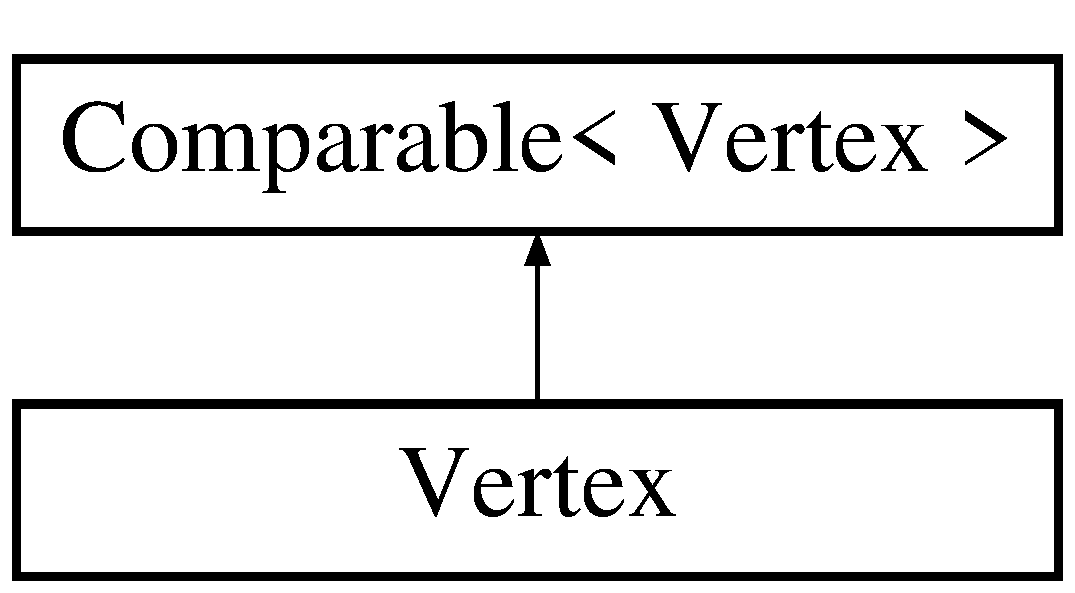
\includegraphics[height=2.000000cm]{class_vertex}
\end{center}
\end{figure}
\subsection*{Public Member Functions}
\begin{DoxyCompactItemize}
\item 
\hyperlink{class_vertex_a9cad0b2dfe2d2d0979d47b2be8325598}{Vertex} (String vertex\+Id)
\begin{DoxyCompactList}\small\item\em constructs a new vertex with the given vertex\+I\+D \end{DoxyCompactList}\item 
void \hyperlink{class_vertex_a36d64c57d236fb0b9c059e2584b53496}{add\+Adjacency} (\hyperlink{class_edge}{Edge} edge)
\begin{DoxyCompactList}\small\item\em adds the given vertex as an adjacency \end{DoxyCompactList}\item 
void \hyperlink{class_vertex_ae9ab92525b737f12bf6ed806d7d3a749}{set\+Vertex\+I\+D} (String I\+D)
\begin{DoxyCompactList}\small\item\em sets the \hyperlink{class_vertex}{Vertex}'s I\+D \end{DoxyCompactList}\item 
void \hyperlink{class_vertex_a98183e2dab0e6b001de3e07d5dd881a3}{set\+Latitude} (int lat)
\begin{DoxyCompactList}\small\item\em sets the latitude coordinate for the \hyperlink{class_vertex}{Vertex} \end{DoxyCompactList}\item 
void \hyperlink{class_vertex_a29dca66870088075feb30929f2908cf4}{set\+Longitude} (int lon)
\begin{DoxyCompactList}\small\item\em sets the longitude coordinate for the \hyperlink{class_vertex}{Vertex} \end{DoxyCompactList}\item 
void \hyperlink{class_vertex_a5d438de1e0b630a74195c816216f092e}{set\+Min\+Distance} (int min)
\begin{DoxyCompactList}\small\item\em sets the minimul distance for the \hyperlink{class_vertex}{Vertex} \end{DoxyCompactList}\item 
void \hyperlink{class_vertex_aae1304e9e84e3cc4dc5c58e12909ee2b}{set\+Prev\+Vertex} (String prev)
\begin{DoxyCompactList}\small\item\em sets the previous \hyperlink{class_vertex}{Vertex}'s previous \hyperlink{class_vertex}{Vertex} \end{DoxyCompactList}\item 
Array\+List$<$ \hyperlink{class_edge}{Edge} $>$ \hyperlink{class_vertex_a0e50bba961059c18d09eae9e4e7ddae6}{get\+Adjacencies} ()
\begin{DoxyCompactList}\small\item\em returns the \hyperlink{class_vertex}{Vertex}'s adjacent Vertexes \end{DoxyCompactList}\item 
String \hyperlink{class_vertex_a90c55a439ee38096f6793d8b53213927}{get\+Vertex\+I\+D} ()
\begin{DoxyCompactList}\small\item\em returns the \hyperlink{class_vertex}{Vertex}'s I\+D \end{DoxyCompactList}\item 
int \hyperlink{class_vertex_a1e30dae20c0f1e9583072b73261fd671}{get\+Latitude} ()
\begin{DoxyCompactList}\small\item\em returns the \hyperlink{class_vertex}{Vertex}'s latitude coordinate \end{DoxyCompactList}\item 
int \hyperlink{class_vertex_a9cc090eee3ea349c68d721e9d447e6c4}{get\+Longitude} ()
\begin{DoxyCompactList}\small\item\em returns the \hyperlink{class_vertex}{Vertex}'s longitude coordinate \end{DoxyCompactList}\item 
int \hyperlink{class_vertex_a184927c05667f9bd103f8ae3ed0d49c6}{get\+Min\+Distance} ()
\begin{DoxyCompactList}\small\item\em returns the \hyperlink{class_vertex}{Vertex}'s min\+Distance \end{DoxyCompactList}\item 
String \hyperlink{class_vertex_adc8513a28f00e0b38d99cdee8229fe06}{get\+Prev\+Vertex} ()
\begin{DoxyCompactList}\small\item\em returns the \hyperlink{class_vertex}{Vertex} previous to the this \hyperlink{class_vertex}{Vertex} \end{DoxyCompactList}\item 
\hypertarget{class_vertex_a7dcf0fc40eacb7e21a8f12682b9be8d4}{int {\bfseries compare\+To} (\hyperlink{class_vertex}{Vertex} vert)}\label{class_vertex_a7dcf0fc40eacb7e21a8f12682b9be8d4}

\end{DoxyCompactItemize}


\subsection{Constructor \& Destructor Documentation}
\hypertarget{class_vertex_a9cad0b2dfe2d2d0979d47b2be8325598}{\index{Vertex@{Vertex}!Vertex@{Vertex}}
\index{Vertex@{Vertex}!Vertex@{Vertex}}
\subsubsection[{Vertex}]{\setlength{\rightskip}{0pt plus 5cm}Vertex.\+Vertex (
\begin{DoxyParamCaption}
\item[{String}]{vertex\+Id}
\end{DoxyParamCaption}
)\hspace{0.3cm}{\ttfamily [inline]}}}\label{class_vertex_a9cad0b2dfe2d2d0979d47b2be8325598}


constructs a new vertex with the given vertex\+I\+D 


\begin{DoxyParams}{Parameters}
{\em String} & vertex\+Id which expects the I\+D for the vertex \\
\hline
\end{DoxyParams}


\subsection{Member Function Documentation}
\hypertarget{class_vertex_a36d64c57d236fb0b9c059e2584b53496}{\index{Vertex@{Vertex}!add\+Adjacency@{add\+Adjacency}}
\index{add\+Adjacency@{add\+Adjacency}!Vertex@{Vertex}}
\subsubsection[{add\+Adjacency}]{\setlength{\rightskip}{0pt plus 5cm}void Vertex.\+add\+Adjacency (
\begin{DoxyParamCaption}
\item[{{\bf Edge}}]{edge}
\end{DoxyParamCaption}
)\hspace{0.3cm}{\ttfamily [inline]}}}\label{class_vertex_a36d64c57d236fb0b9c059e2584b53496}


adds the given vertex as an adjacency 


\begin{DoxyParams}{Parameters}
{\em \hyperlink{class_vertex}{Vertex}} & vertex which expects the vertex that is adjacent \\
\hline
\end{DoxyParams}
\begin{DoxyReturn}{Returns}
void 
\end{DoxyReturn}
\hypertarget{class_vertex_a0e50bba961059c18d09eae9e4e7ddae6}{\index{Vertex@{Vertex}!get\+Adjacencies@{get\+Adjacencies}}
\index{get\+Adjacencies@{get\+Adjacencies}!Vertex@{Vertex}}
\subsubsection[{get\+Adjacencies}]{\setlength{\rightskip}{0pt plus 5cm}Array\+List$<${\bf Edge}$>$ Vertex.\+get\+Adjacencies (
\begin{DoxyParamCaption}
{}
\end{DoxyParamCaption}
)\hspace{0.3cm}{\ttfamily [inline]}}}\label{class_vertex_a0e50bba961059c18d09eae9e4e7ddae6}


returns the \hyperlink{class_vertex}{Vertex}'s adjacent Vertexes 

\begin{DoxyReturn}{Returns}
Array\+List$<$\+Vertex$>$ 
\end{DoxyReturn}
\hypertarget{class_vertex_a1e30dae20c0f1e9583072b73261fd671}{\index{Vertex@{Vertex}!get\+Latitude@{get\+Latitude}}
\index{get\+Latitude@{get\+Latitude}!Vertex@{Vertex}}
\subsubsection[{get\+Latitude}]{\setlength{\rightskip}{0pt plus 5cm}int Vertex.\+get\+Latitude (
\begin{DoxyParamCaption}
{}
\end{DoxyParamCaption}
)\hspace{0.3cm}{\ttfamily [inline]}}}\label{class_vertex_a1e30dae20c0f1e9583072b73261fd671}


returns the \hyperlink{class_vertex}{Vertex}'s latitude coordinate 

\begin{DoxyReturn}{Returns}
double 
\end{DoxyReturn}
\hypertarget{class_vertex_a9cc090eee3ea349c68d721e9d447e6c4}{\index{Vertex@{Vertex}!get\+Longitude@{get\+Longitude}}
\index{get\+Longitude@{get\+Longitude}!Vertex@{Vertex}}
\subsubsection[{get\+Longitude}]{\setlength{\rightskip}{0pt plus 5cm}int Vertex.\+get\+Longitude (
\begin{DoxyParamCaption}
{}
\end{DoxyParamCaption}
)\hspace{0.3cm}{\ttfamily [inline]}}}\label{class_vertex_a9cc090eee3ea349c68d721e9d447e6c4}


returns the \hyperlink{class_vertex}{Vertex}'s longitude coordinate 

\begin{DoxyReturn}{Returns}
double 
\end{DoxyReturn}
\hypertarget{class_vertex_a184927c05667f9bd103f8ae3ed0d49c6}{\index{Vertex@{Vertex}!get\+Min\+Distance@{get\+Min\+Distance}}
\index{get\+Min\+Distance@{get\+Min\+Distance}!Vertex@{Vertex}}
\subsubsection[{get\+Min\+Distance}]{\setlength{\rightskip}{0pt plus 5cm}int Vertex.\+get\+Min\+Distance (
\begin{DoxyParamCaption}
{}
\end{DoxyParamCaption}
)\hspace{0.3cm}{\ttfamily [inline]}}}\label{class_vertex_a184927c05667f9bd103f8ae3ed0d49c6}


returns the \hyperlink{class_vertex}{Vertex}'s min\+Distance 

\begin{DoxyReturn}{Returns}
int 
\end{DoxyReturn}
\hypertarget{class_vertex_adc8513a28f00e0b38d99cdee8229fe06}{\index{Vertex@{Vertex}!get\+Prev\+Vertex@{get\+Prev\+Vertex}}
\index{get\+Prev\+Vertex@{get\+Prev\+Vertex}!Vertex@{Vertex}}
\subsubsection[{get\+Prev\+Vertex}]{\setlength{\rightskip}{0pt plus 5cm}String Vertex.\+get\+Prev\+Vertex (
\begin{DoxyParamCaption}
{}
\end{DoxyParamCaption}
)\hspace{0.3cm}{\ttfamily [inline]}}}\label{class_vertex_adc8513a28f00e0b38d99cdee8229fe06}


returns the \hyperlink{class_vertex}{Vertex} previous to the this \hyperlink{class_vertex}{Vertex} 

\begin{DoxyReturn}{Returns}
\hyperlink{class_vertex}{Vertex} 
\end{DoxyReturn}
\hypertarget{class_vertex_a90c55a439ee38096f6793d8b53213927}{\index{Vertex@{Vertex}!get\+Vertex\+I\+D@{get\+Vertex\+I\+D}}
\index{get\+Vertex\+I\+D@{get\+Vertex\+I\+D}!Vertex@{Vertex}}
\subsubsection[{get\+Vertex\+I\+D}]{\setlength{\rightskip}{0pt plus 5cm}String Vertex.\+get\+Vertex\+I\+D (
\begin{DoxyParamCaption}
{}
\end{DoxyParamCaption}
)\hspace{0.3cm}{\ttfamily [inline]}}}\label{class_vertex_a90c55a439ee38096f6793d8b53213927}


returns the \hyperlink{class_vertex}{Vertex}'s I\+D 

\begin{DoxyReturn}{Returns}
String 
\end{DoxyReturn}
\hypertarget{class_vertex_a98183e2dab0e6b001de3e07d5dd881a3}{\index{Vertex@{Vertex}!set\+Latitude@{set\+Latitude}}
\index{set\+Latitude@{set\+Latitude}!Vertex@{Vertex}}
\subsubsection[{set\+Latitude}]{\setlength{\rightskip}{0pt plus 5cm}void Vertex.\+set\+Latitude (
\begin{DoxyParamCaption}
\item[{int}]{lat}
\end{DoxyParamCaption}
)\hspace{0.3cm}{\ttfamily [inline]}}}\label{class_vertex_a98183e2dab0e6b001de3e07d5dd881a3}


sets the latitude coordinate for the \hyperlink{class_vertex}{Vertex} 


\begin{DoxyParams}{Parameters}
{\em double} & lat which expects a latitude coordinate \\
\hline
\end{DoxyParams}
\begin{DoxyReturn}{Returns}
void 
\end{DoxyReturn}
\hypertarget{class_vertex_a29dca66870088075feb30929f2908cf4}{\index{Vertex@{Vertex}!set\+Longitude@{set\+Longitude}}
\index{set\+Longitude@{set\+Longitude}!Vertex@{Vertex}}
\subsubsection[{set\+Longitude}]{\setlength{\rightskip}{0pt plus 5cm}void Vertex.\+set\+Longitude (
\begin{DoxyParamCaption}
\item[{int}]{lon}
\end{DoxyParamCaption}
)\hspace{0.3cm}{\ttfamily [inline]}}}\label{class_vertex_a29dca66870088075feb30929f2908cf4}


sets the longitude coordinate for the \hyperlink{class_vertex}{Vertex} 


\begin{DoxyParams}{Parameters}
{\em double} & lon which expects a longitude coordinate \\
\hline
\end{DoxyParams}
\begin{DoxyReturn}{Returns}
void 
\end{DoxyReturn}
\hypertarget{class_vertex_a5d438de1e0b630a74195c816216f092e}{\index{Vertex@{Vertex}!set\+Min\+Distance@{set\+Min\+Distance}}
\index{set\+Min\+Distance@{set\+Min\+Distance}!Vertex@{Vertex}}
\subsubsection[{set\+Min\+Distance}]{\setlength{\rightskip}{0pt plus 5cm}void Vertex.\+set\+Min\+Distance (
\begin{DoxyParamCaption}
\item[{int}]{min}
\end{DoxyParamCaption}
)\hspace{0.3cm}{\ttfamily [inline]}}}\label{class_vertex_a5d438de1e0b630a74195c816216f092e}


sets the minimul distance for the \hyperlink{class_vertex}{Vertex} 


\begin{DoxyParams}{Parameters}
{\em int} & min\+Dist which expects the minimum distance \\
\hline
\end{DoxyParams}
\begin{DoxyReturn}{Returns}
void 
\end{DoxyReturn}
\hypertarget{class_vertex_aae1304e9e84e3cc4dc5c58e12909ee2b}{\index{Vertex@{Vertex}!set\+Prev\+Vertex@{set\+Prev\+Vertex}}
\index{set\+Prev\+Vertex@{set\+Prev\+Vertex}!Vertex@{Vertex}}
\subsubsection[{set\+Prev\+Vertex}]{\setlength{\rightskip}{0pt plus 5cm}void Vertex.\+set\+Prev\+Vertex (
\begin{DoxyParamCaption}
\item[{String}]{prev}
\end{DoxyParamCaption}
)\hspace{0.3cm}{\ttfamily [inline]}}}\label{class_vertex_aae1304e9e84e3cc4dc5c58e12909ee2b}


sets the previous \hyperlink{class_vertex}{Vertex}'s previous \hyperlink{class_vertex}{Vertex} 


\begin{DoxyParams}{Parameters}
{\em \hyperlink{class_vertex}{Vertex}} & prev which expects the \hyperlink{class_vertex}{Vertex} previous to this one \\
\hline
\end{DoxyParams}
\begin{DoxyReturn}{Returns}
void 
\end{DoxyReturn}
\hypertarget{class_vertex_ae9ab92525b737f12bf6ed806d7d3a749}{\index{Vertex@{Vertex}!set\+Vertex\+I\+D@{set\+Vertex\+I\+D}}
\index{set\+Vertex\+I\+D@{set\+Vertex\+I\+D}!Vertex@{Vertex}}
\subsubsection[{set\+Vertex\+I\+D}]{\setlength{\rightskip}{0pt plus 5cm}void Vertex.\+set\+Vertex\+I\+D (
\begin{DoxyParamCaption}
\item[{String}]{I\+D}
\end{DoxyParamCaption}
)\hspace{0.3cm}{\ttfamily [inline]}}}\label{class_vertex_ae9ab92525b737f12bf6ed806d7d3a749}


sets the \hyperlink{class_vertex}{Vertex}'s I\+D 


\begin{DoxyParams}{Parameters}
{\em String} & I\+D which expects the I\+D for the vertex \\
\hline
\end{DoxyParams}
\begin{DoxyReturn}{Returns}
void 
\end{DoxyReturn}


The documentation for this class was generated from the following file\+:\begin{DoxyCompactItemize}
\item 
\hyperlink{_vertex_8java}{Vertex.\+java}\end{DoxyCompactItemize}

\chapter{File Documentation}
\hypertarget{_find_shortest_road_path_8java}{\section{Find\+Shortest\+Road\+Path.\+java File Reference}
\label{_find_shortest_road_path_8java}\index{Find\+Shortest\+Road\+Path.\+java@{Find\+Shortest\+Road\+Path.\+java}}
}


Class \hyperlink{class_find_shortest_road_path}{Find\+Shortest\+Road\+Path} is used to gather user input data and initialize the graph. It will then perform \hyperlink{class_dijkstra}{Dijkstra}'s Algorithm on the graph and save the results to a text file.  


\subsection*{Classes}
\begin{DoxyCompactItemize}
\item 
class \hyperlink{class_find_shortest_road_path}{Find\+Shortest\+Road\+Path}
\end{DoxyCompactItemize}


\subsection{Detailed Description}
Class \hyperlink{class_find_shortest_road_path}{Find\+Shortest\+Road\+Path} is used to gather user input data and initialize the graph. It will then perform \hyperlink{class_dijkstra}{Dijkstra}'s Algorithm on the graph and save the results to a text file. 

\begin{DoxyAuthor}{Author}
Joshua Lewis Eaton 
\end{DoxyAuthor}
\begin{DoxyDate}{Date}
December 5, 2014 
\end{DoxyDate}

\hypertarget{_graph_8java}{\section{Graph.\+java File Reference}
\label{_graph_8java}\index{Graph.\+java@{Graph.\+java}}
}


Class \hyperlink{class_graph}{Graph} defines a graph that is made of vertexes and edges, the underlying implementation is a hashmap.  


\subsection*{Classes}
\begin{DoxyCompactItemize}
\item 
class \hyperlink{class_graph}{Graph}
\end{DoxyCompactItemize}


\subsection{Detailed Description}
Class \hyperlink{class_graph}{Graph} defines a graph that is made of vertexes and edges, the underlying implementation is a hashmap. 

\begin{DoxyAuthor}{Author}
Joshua Lewis Eaton 
\end{DoxyAuthor}
\begin{DoxyDate}{Date}
December 5, 2014 
\end{DoxyDate}

\hypertarget{_graph_initializer_8java}{\section{Graph\+Initializer.\+java File Reference}
\label{_graph_initializer_8java}\index{Graph\+Initializer.\+java@{Graph\+Initializer.\+java}}
}


Class \hyperlink{class_graph_initializer}{Graph\+Initializer} is used to fill the \hyperlink{class_graph}{Graph} with the data from input files.  


\subsection*{Classes}
\begin{DoxyCompactItemize}
\item 
class \hyperlink{class_graph_initializer}{Graph\+Initializer}
\end{DoxyCompactItemize}


\subsection{Detailed Description}
Class \hyperlink{class_graph_initializer}{Graph\+Initializer} is used to fill the \hyperlink{class_graph}{Graph} with the data from input files. 

\begin{DoxyAuthor}{Author}
Joshua Lewis Eaton 
\end{DoxyAuthor}
\begin{DoxyDate}{Date}
December 5, 2014 
\end{DoxyDate}

\hypertarget{_vertex_8java}{\section{Vertex.\+java File Reference}
\label{_vertex_8java}\index{Vertex.\+java@{Vertex.\+java}}
}


Class \hyperlink{class_vertex}{Vertex} defines a \hyperlink{class_vertex}{Vertex} in relation to a \hyperlink{class_graph}{Graph}.  


\subsection*{Classes}
\begin{DoxyCompactItemize}
\item 
class \hyperlink{class_vertex}{Vertex}
\end{DoxyCompactItemize}


\subsection{Detailed Description}
Class \hyperlink{class_vertex}{Vertex} defines a \hyperlink{class_vertex}{Vertex} in relation to a \hyperlink{class_graph}{Graph}. 

\begin{DoxyAuthor}{Author}
Joshua Lewis Eaton 
\end{DoxyAuthor}
\begin{DoxyDate}{Date}
December 5, 2014 
\end{DoxyDate}

%--- End generated contents ---

% Index
\newpage
\phantomsection
\addcontentsline{toc}{chapter}{Index}
\printindex

\end{document}
